\documentclass[tikz]{standalone}
\usepackage{tikz}
\usetikzlibrary{automata}

\begin{document}
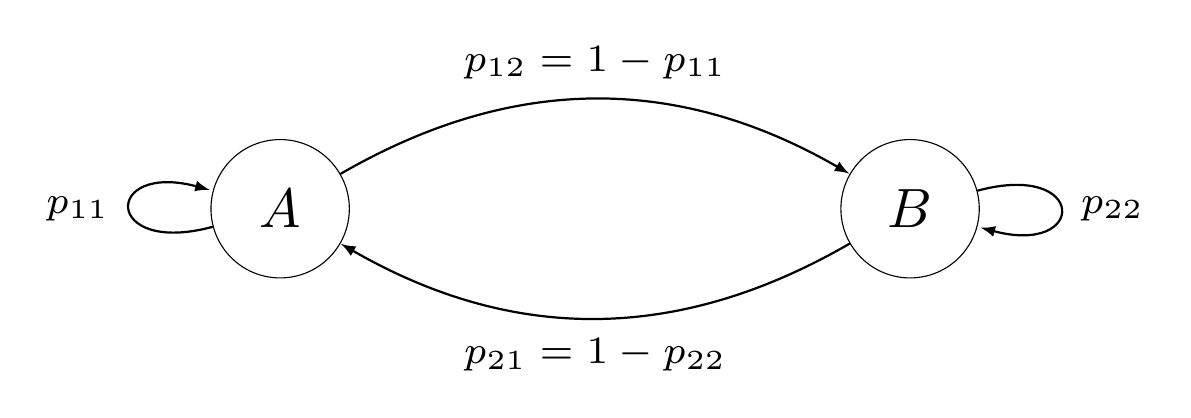
\begin{tikzpicture}[scale=2, transform shape, line cap=round, line join=round, node distance=4cm,
    ->, >=latex, auto, every edge/.append style={thick}] % transform shape

  \node[state] (1) {$A$};
  \node[state] (2) [right of=1]  {$B$};

  \path (1) edge[loop left] node{\scriptsize{$p_{11}$}} (1)
  edge[bend left] node{\scriptsize{$p_{12} = 1 - p_{11}$}} (2)
  (2) edge[loop right] node{\scriptsize{$p_{22}$}} (2)
  edge[bend left] node{\scriptsize{$p_{21} = 1 - p_{22}$}} (1);
\end{tikzpicture}
\end{document}
